\documentclass{ximera}

%\usepackage{todonotes}

\newcommand{\todo}{}

\usepackage{esint} % for \oiint
\ifxake%%https://math.meta.stackexchange.com/questions/9973/how-do-you-render-a-closed-surface-double-integral
\renewcommand{\oiint}{{\large\bigcirc}\kern-1.56em\iint}
\fi


\graphicspath{
  {./}
  {ximeraTutorial/}
  {basicPhilosophy/}
  {functionsOfSeveralVariables/}
  {normalVectors/}
  {lagrangeMultipliers/}
  {vectorFields/}
  {greensTheorem/}
  {shapeOfThingsToCome/}
  {dotProducts/}
  {partialDerivativesAndTheGradientVector/}
  {../productAndQuotientRules/exercises/}
  {../normalVectors/exercisesParametricPlots/}
  {../continuityOfFunctionsOfSeveralVariables/exercises/}
  {../partialDerivativesAndTheGradientVector/exercises/}
  {../directionalDerivativeAndChainRule/exercises/}
  {../commonCoordinates/exercisesCylindricalCoordinates/}
  {../commonCoordinates/exercisesSphericalCoordinates/}
  {../greensTheorem/exercisesCurlAndLineIntegrals/}
  {../greensTheorem/exercisesDivergenceAndLineIntegrals/}
  {../shapeOfThingsToCome/exercisesDivergenceTheorem/}
  {../greensTheorem/}
  {../shapeOfThingsToCome/}
  {../separableDifferentialEquations/exercises/}
  {vectorFields/}
}

\newcommand{\mooculus}{\textsf{\textbf{MOOC}\textnormal{\textsf{ULUS}}}}

\usepackage{tkz-euclide}
\usepackage{tikz}
\usepackage{tikz-cd}
\usetikzlibrary{arrows}
\tikzset{>=stealth,commutative diagrams/.cd,
  arrow style=tikz,diagrams={>=stealth}} %% cool arrow head
\tikzset{shorten <>/.style={ shorten >=#1, shorten <=#1 } } %% allows shorter vectors

\usetikzlibrary{backgrounds} %% for boxes around graphs
\usetikzlibrary{shapes,positioning}  %% Clouds and stars
\usetikzlibrary{matrix} %% for matrix
\usepgfplotslibrary{polar} %% for polar plots
\usepgfplotslibrary{fillbetween} %% to shade area between curves in TikZ
%\usetkzobj{all}
\usepackage[makeroom]{cancel} %% for strike outs
%\usepackage{mathtools} %% for pretty underbrace % Breaks Ximera
%\usepackage{multicol}
\usepackage{pgffor} %% required for integral for loops



%% http://tex.stackexchange.com/questions/66490/drawing-a-tikz-arc-specifying-the-center
%% Draws beach ball
\tikzset{pics/carc/.style args={#1:#2:#3}{code={\draw[pic actions] (#1:#3) arc(#1:#2:#3);}}}



\usepackage{array}
\setlength{\extrarowheight}{+.1cm}
\newdimen\digitwidth
\settowidth\digitwidth{9}
\def\divrule#1#2{
\noalign{\moveright#1\digitwidth
\vbox{\hrule width#2\digitwidth}}}




% \newcommand{\RR}{\mathbb R}
% \newcommand{\R}{\mathbb R}
% \newcommand{\N}{\mathbb N}
% \newcommand{\Z}{\mathbb Z}

\newcommand{\sagemath}{\textsf{SageMath}}


%\renewcommand{\d}{\,d\!}
%\renewcommand{\d}{\mathop{}\!d}
%\newcommand{\dd}[2][]{\frac{\d #1}{\d #2}}
%\newcommand{\pp}[2][]{\frac{\partial #1}{\partial #2}}
% \renewcommand{\l}{\ell}
%\newcommand{\ddx}{\frac{d}{\d x}}

% \newcommand{\zeroOverZero}{\ensuremath{\boldsymbol{\tfrac{0}{0}}}}
%\newcommand{\inftyOverInfty}{\ensuremath{\boldsymbol{\tfrac{\infty}{\infty}}}}
%\newcommand{\zeroOverInfty}{\ensuremath{\boldsymbol{\tfrac{0}{\infty}}}}
%\newcommand{\zeroTimesInfty}{\ensuremath{\small\boldsymbol{0\cdot \infty}}}
%\newcommand{\inftyMinusInfty}{\ensuremath{\small\boldsymbol{\infty - \infty}}}
%\newcommand{\oneToInfty}{\ensuremath{\boldsymbol{1^\infty}}}
%\newcommand{\zeroToZero}{\ensuremath{\boldsymbol{0^0}}}
%\newcommand{\inftyToZero}{\ensuremath{\boldsymbol{\infty^0}}}



% \newcommand{\numOverZero}{\ensuremath{\boldsymbol{\tfrac{\#}{0}}}}
% \newcommand{\dfn}{\textbf}
% \newcommand{\unit}{\,\mathrm}
% \newcommand{\unit}{\mathop{}\!\mathrm}
% \newcommand{\eval}[1]{\bigg[ #1 \bigg]}
% \newcommand{\seq}[1]{\left( #1 \right)}
% \renewcommand{\epsilon}{\varepsilon}
% \renewcommand{\phi}{\varphi}


% \renewcommand{\iff}{\Leftrightarrow}

% \DeclareMathOperator{\arccot}{arccot}
% \DeclareMathOperator{\arcsec}{arcsec}
% \DeclareMathOperator{\arccsc}{arccsc}
% \DeclareMathOperator{\si}{Si}
% \DeclareMathOperator{\scal}{scal}
% \DeclareMathOperator{\sign}{sign}


%% \newcommand{\tightoverset}[2]{% for arrow vec
%%   \mathop{#2}\limits^{\vbox to -.5ex{\kern-0.75ex\hbox{$#1$}\vss}}}
% \newcommand{\arrowvec}[1]{{\overset{\rightharpoonup}{#1}}}
% \renewcommand{\vec}[1]{\arrowvec{\mathbf{#1}}}
% \renewcommand{\vec}[1]{{\overset{\boldsymbol{\rightharpoonup}}{\mathbf{#1}}}}

% \newcommand{\point}[1]{\left(#1\right)} %this allows \vector{ to be changed to \vector{ with a quick find and replace
% \newcommand{\pt}[1]{\mathbf{#1}} %this allows \vec{ to be changed to \vec{ with a quick find and replace
% \newcommand{\Lim}[2]{\lim_{\point{#1} \to \point{#2}}} %Bart, I changed this to point since I want to use it.  It runs through both of the exercise and exerciseE files in limits section, which is why it was in each document to start with.

% \DeclareMathOperator{\proj}{\mathbf{proj}}
% \newcommand{\veci}{{\boldsymbol{\hat{\imath}}}}
% \newcommand{\vecj}{{\boldsymbol{\hat{\jmath}}}}
% \newcommand{\veck}{{\boldsymbol{\hat{k}}}}
% \newcommand{\vecl}{\vec{\boldsymbol{\l}}}
% \newcommand{\uvec}[1]{\mathbf{\hat{#1}}}
% \newcommand{\utan}{\mathbf{\hat{t}}}
% \newcommand{\unormal}{\mathbf{\hat{n}}}
% \newcommand{\ubinormal}{\mathbf{\hat{b}}}

% \newcommand{\dotp}{\bullet}
% \newcommand{\cross}{\boldsymbol\times}
% \newcommand{\grad}{\boldsymbol\nabla}
% \newcommand{\divergence}{\grad\dotp}
% \newcommand{\curl}{\grad\cross}
%\DeclareMathOperator{\divergence}{divergence}
%\DeclareMathOperator{\curl}[1]{\grad\cross #1}
% \newcommand{\lto}{\mathop{\longrightarrow\,}\limits}

% \renewcommand{\bar}{\overline}

\colorlet{textColor}{black}
\colorlet{background}{white}
\colorlet{penColor}{blue!50!black} % Color of a curve in a plot
\colorlet{penColor2}{red!50!black}% Color of a curve in a plot
\colorlet{penColor3}{red!50!blue} % Color of a curve in a plot
\colorlet{penColor4}{green!50!black} % Color of a curve in a plot
\colorlet{penColor5}{orange!80!black} % Color of a curve in a plot
\colorlet{penColor6}{yellow!70!black} % Color of a curve in a plot
\colorlet{fill1}{penColor!20} % Color of fill in a plot
\colorlet{fill2}{penColor2!20} % Color of fill in a plot
\colorlet{fillp}{fill1} % Color of positive area
\colorlet{filln}{penColor2!20} % Color of negative area
\colorlet{fill3}{penColor3!20} % Fill
\colorlet{fill4}{penColor4!20} % Fill
\colorlet{fill5}{penColor5!20} % Fill
\colorlet{gridColor}{gray!50} % Color of grid in a plot

\newcommand{\surfaceColor}{violet}
\newcommand{\surfaceColorTwo}{redyellow}
\newcommand{\sliceColor}{greenyellow}




\pgfmathdeclarefunction{gauss}{2}{% gives gaussian
  \pgfmathparse{1/(#2*sqrt(2*pi))*exp(-((x-#1)^2)/(2*#2^2))}%
}


%%%%%%%%%%%%%
%% Vectors
%%%%%%%%%%%%%

%% Simple horiz vectors
\renewcommand{\vector}[1]{\left\langle #1\right\rangle}


%% %% Complex Horiz Vectors with angle brackets
%% \makeatletter
%% \renewcommand{\vector}[2][ , ]{\left\langle%
%%   \def\nextitem{\def\nextitem{#1}}%
%%   \@for \el:=#2\do{\nextitem\el}\right\rangle%
%% }
%% \makeatother

%% %% Vertical Vectors
%% \def\vector#1{\begin{bmatrix}\vecListA#1,,\end{bmatrix}}
%% \def\vecListA#1,{\if,#1,\else #1\cr \expandafter \vecListA \fi}

%%%%%%%%%%%%%
%% End of vectors
%%%%%%%%%%%%%

%\newcommand{\fullwidth}{}
%\newcommand{\normalwidth}{}



%% makes a snazzy t-chart for evaluating functions
%\newenvironment{tchart}{\rowcolors{2}{}{background!90!textColor}\array}{\endarray}

%%This is to help with formatting on future title pages.
\newenvironment{sectionOutcomes}{}{}



%% Flowchart stuff
%\tikzstyle{startstop} = [rectangle, rounded corners, minimum width=3cm, minimum height=1cm,text centered, draw=black]
%\tikzstyle{question} = [rectangle, minimum width=3cm, minimum height=1cm, text centered, draw=black]
%\tikzstyle{decision} = [trapezium, trapezium left angle=70, trapezium right angle=110, minimum width=3cm, minimum height=1cm, text centered, draw=black]
%\tikzstyle{question} = [rectangle, rounded corners, minimum width=3cm, minimum height=1cm,text centered, draw=black]
%\tikzstyle{process} = [rectangle, minimum width=3cm, minimum height=1cm, text centered, draw=black]
%\tikzstyle{decision} = [trapezium, trapezium left angle=70, trapezium right angle=110, minimum width=3cm, minimum height=1cm, text centered, draw=black]


\title{Up and Down}

\begin{document}

\begin{abstract}
stretch the range
\end{abstract}
\maketitle











Let $W(y)$ be a function with its domain and range.

Let $K(r)$ be defined as $K(r) = 2 W(r)$ with its induced domain and range.


Then the domain of $K$ is

\begin{multipleChoice}
\choice {the domain of $W$ stretched by $2$}
\choice {the domain of $W$ compressed by $\tfrac{1}{2}$}
\choice[correct] {the same as for $W$}
\end{multipleChoice}

The induced domain of $K$ is equal to the domain of $W$.  The coefficient $2$ is multiplying the function values of $W$.



\begin{question}


Suppose $K(r) = 2 W(r)$ and $W(4) = 6$.  Then which of the following is true?

\begin{multipleChoice}
\choice {$K(2) = 6$}
\choice[correct] {$K(4) = 12$}
\choice {$K(2) = 3$}
\choice {$K(4) = 3$}
\end{multipleChoice}


\end{question}







\begin{example} Stretching Vertically




Graph of $y = m(f)$.

\begin{image}
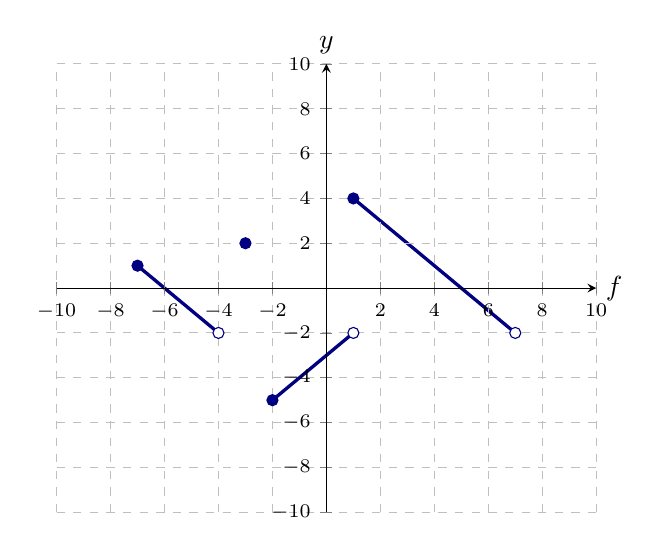
\begin{tikzpicture}
	\begin{axis}[
            domain=-10:10, ymax=10, xmax=10, ymin=-10, xmin=-10,
            axis lines =center, xlabel=$f$, ylabel=$y$, grid = major, grid style={dashed},
            ytick={-10,-8,-6,-4,-2,2,4,6,8,10},
            xtick={-10,-8,-6,-4,-2,2,4,6,8,10},
            ticklabel style={font=\scriptsize},
            every axis y label/.style={at=(current axis.above origin),anchor=south},
            every axis x label/.style={at=(current axis.right of origin),anchor=west},
            axis on top
          ]
          
	\addplot [draw=penColor,very thick,smooth,domain=(-7:-4)] {-x-6};
	\addplot [draw=penColor,very thick,smooth,domain=(-2:1)] {x-3};
	\addplot [draw=penColor,very thick,smooth,domain=(1:7)] {-x+5};

	\addplot[color=penColor,only marks,mark=*] coordinates{(-3,2)}; 
	
	\addplot[color=penColor,only marks,mark=*] coordinates{(-7,1)}; 
	\addplot[color=penColor,fill=white,only marks,mark=*] coordinates{(-4,-2)}; 
	\addplot[color=penColor,only marks,mark=*] coordinates{(-2,-5)}; 
	\addplot[color=penColor,fill=white, only marks,mark=*] coordinates{(1,-2)}; 
	\addplot[color=penColor,only marks,mark=*] coordinates{(1,4)}; 
	\addplot[color=penColor,fill=white,only marks,mark=*] coordinates{(7,-2)}; 


    \end{axis}
\end{tikzpicture}
\end{image}


$m$ has two zeros: $-6$ and $\answer{5}$. These are represented by intercepts in the left and right line segments. \\
$m$ has a global minimum represent by the left endpoint of the middle line segment. \\
$m$ has a global maximum represent by the left endpoint of the right line segment.





Graph of $z = P(t) = 2 \, m(t)$.

\begin{image}
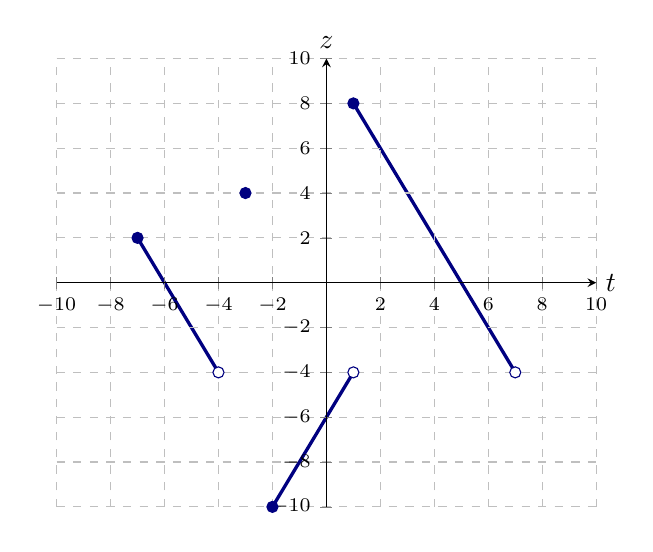
\begin{tikzpicture}
	\begin{axis}[
            domain=-10:10, ymax=10, xmax=10, ymin=-10, xmin=-10,
            axis lines =center, xlabel=$t$, ylabel=$z$, grid = major, grid style={dashed},
            ytick={-10,-8,-6,-4,-2,2,4,6,8,10},
            xtick={-10,-8,-6,-4,-2,2,4,6,8,10},
            ticklabel style={font=\scriptsize},
            every axis y label/.style={at=(current axis.above origin),anchor=south},
            every axis x label/.style={at=(current axis.right of origin),anchor=west},
            axis on top
          ]
          
	\addplot [draw=penColor,very thick,smooth,domain=(-7:-4)] {2*(-x-6)};
  \addplot [draw=penColor,very thick,smooth,domain=(-2:1)] {2*(x-3)};
  \addplot [draw=penColor,very thick,smooth,domain=(1:7)] {2*(-x+5)};

  \addplot[color=penColor,only marks,mark=*] coordinates{(-3,4)}; 
  
  \addplot[color=penColor,only marks,mark=*] coordinates{(-7,2)}; 
  \addplot[color=penColor,fill=white,only marks,mark=*] coordinates{(-4,-4)}; 
  \addplot[color=penColor,only marks,mark=*] coordinates{(-2,-10)}; 
  \addplot[color=penColor,fill=white,only marks,mark=*] coordinates{(1,-4)}; 
  \addplot[color=penColor,only marks,mark=*] coordinates{(1,8)}; 
  \addplot[color=penColor,fill=white,only marks,mark=*] coordinates{(7,-4)}; 


    \end{axis}
\end{tikzpicture}
\end{image}




\begin{itemize}

\item The domain of $P$ is $\left[\answer{-7},\answer{-4}\right) \cup \{3\} \cup [-2,7)$, equal to the domain of $m$. The domain remains the same, since the $2$ was outside the domain parentheses in the formula for $m$. The $2$ is multiplying the function values.
\item $P$ has two zeros: $-6$ and $5$. These are represented by intercepts in the left and right line segments. (Because, $2 \cdot 0 = 0$.) \\
\item $P$ has a global minimum represented by the left endpoint of the middle line segment. \\
\item $P$ has a global maximum represented by the left endpoint of the right line segment.

\end{itemize}


\end{example}


Multiplying a function by a positive constant greater than $1$ stetches the graph vertically.  Since stretching $0$ still gives $0$, the intercepts do not change.  Everything is stetched from the intercepts. The intercepts stay pinned where they are.


















Multiplying by a negative constant less than $-1$ does the same thing, but also reflects the graph about the horizontal axis.





\begin{example} Reflecting Vertically




Graph of $y = m(f)$.

\begin{image}
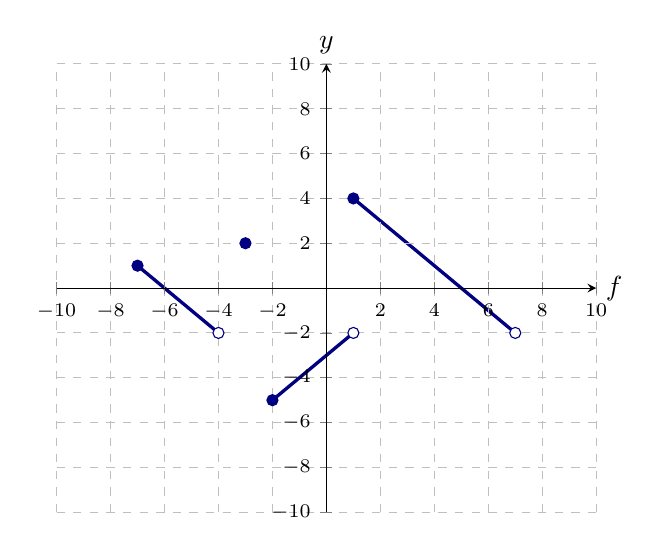
\begin{tikzpicture}
  \begin{axis}[
            domain=-10:10, ymax=10, xmax=10, ymin=-10, xmin=-10,
            axis lines =center, xlabel=$f$, ylabel=$y$, grid = major, grid style={dashed},
            ytick={-10,-8,-6,-4,-2,2,4,6,8,10},
            xtick={-10,-8,-6,-4,-2,2,4,6,8,10},
            ticklabel style={font=\scriptsize},
            every axis y label/.style={at=(current axis.above origin),anchor=south},
            every axis x label/.style={at=(current axis.right of origin),anchor=west},
            axis on top
          ]
          
  \addplot [draw=penColor,very thick,smooth,domain=(-7:-4)] {-x-6};
  \addplot [draw=penColor,very thick,smooth,domain=(-2:1)] {x-3};
  \addplot [draw=penColor,very thick,smooth,domain=(1:7)] {-x+5};

  \addplot[color=penColor,only marks,mark=*] coordinates{(-3,2)}; 
  
  \addplot[color=penColor,only marks,mark=*] coordinates{(-7,1)}; 
  \addplot[color=penColor,fill=white,only marks,mark=*] coordinates{(-4,-2)}; 
  \addplot[color=penColor,only marks,mark=*] coordinates{(-2,-5)}; 
  \addplot[color=penColor,fill=white,only marks,mark=*] coordinates{(1,-2)}; 
  \addplot[color=penColor,only marks,mark=*] coordinates{(1,4)}; 
  \addplot[color=penColor,fill=white,only marks,mark=*] coordinates{(7,-2)}; 


    \end{axis}
\end{tikzpicture}
\end{image}


$m$ has two zeros: $-6$ and $5$. These are represented by intercepts in the left and right line segments. 
$m$ has a global minimum represent by the left endpoint of the middle line segment. 
$m$ has a global maximum represent by the left endpoint of the right line segment.





Graph of $z = B(h) = -2 \, m(h)$.

\begin{image}
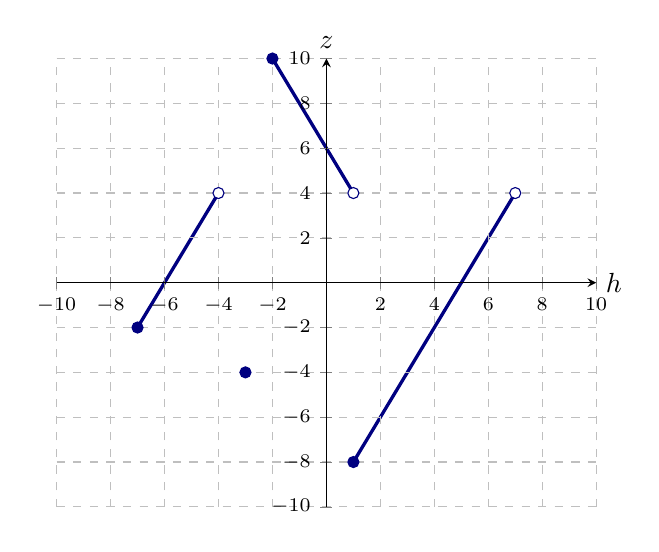
\begin{tikzpicture}
  \begin{axis}[
            domain=-10:10, ymax=10, xmax=10, ymin=-10, xmin=-10,
            axis lines =center, xlabel=$h$, ylabel=$z$, grid = major, grid style={dashed},
            ytick={-10,-8,-6,-4,-2,2,4,6,8,10},
            xtick={-10,-8,-6,-4,-2,2,4,6,8,10},
            ticklabel style={font=\scriptsize},
            every axis y label/.style={at=(current axis.above origin),anchor=south},
            every axis x label/.style={at=(current axis.right of origin),anchor=west},
            axis on top
          ]
          
  \addplot [draw=penColor,very thick,smooth,domain=(-7:-4)] {2*x+12};
  \addplot [draw=penColor,very thick,smooth,domain=(-2:1)] {-2*x+6};
  \addplot [draw=penColor,very thick,smooth,domain=(1:7)] {2*x-10};

  \addplot[color=penColor,only marks,mark=*] coordinates{(-3,-4)}; 
  
  \addplot[color=penColor,only marks,mark=*] coordinates{(-7,-2)}; 
  \addplot[color=penColor,fill=white,only marks,mark=*] coordinates{(-4,4)}; 
  \addplot[color=penColor,only marks,mark=*] coordinates{(-2,10)}; 
  \addplot[color=penColor,fill=white,only marks,mark=*] coordinates{(1,4)}; 
  \addplot[color=penColor,only marks,mark=*] coordinates{(1,-8)}; 
  \addplot[color=penColor,fill=white,only marks,mark=*] coordinates{(7,4)}; 


    \end{axis}
\end{tikzpicture}
\end{image}


The shape has not changed.  It has just been flipped over vertically, about the horizontal axis.

\begin{itemize}

\item The domain of $B$ is $[-7,-4) \cup \{3\} \cup [-2,7)$, equal to the domain of $m$.  The factor, $-2$, was outside the domain parentheses in the formula for $m$.
\item $B$ has two zeros: $\answer{-6}$ and $5$. These are represented by intercepts in the left and right line segments. (Because, $-2 \cdot 0 = 0$.) \\
\item $B$ has a global minimum.  It is represented by the flipped highest dot in the graph of $m$.\\
\item $B$ has a global maximum.  It is represented by the flipped lowest dot in the graph of $m$.

\end{itemize}


\end{example}















Multiplying by a number smaller than $1$, squeezes the graph vertically.  Our word for this is ``compress''.  Multiplying a function by a number between $-1$ and $1$ compresses the graph vertically.




\begin{example} Compressing Vertically




Graph of $y = m(f)$.

\begin{image}
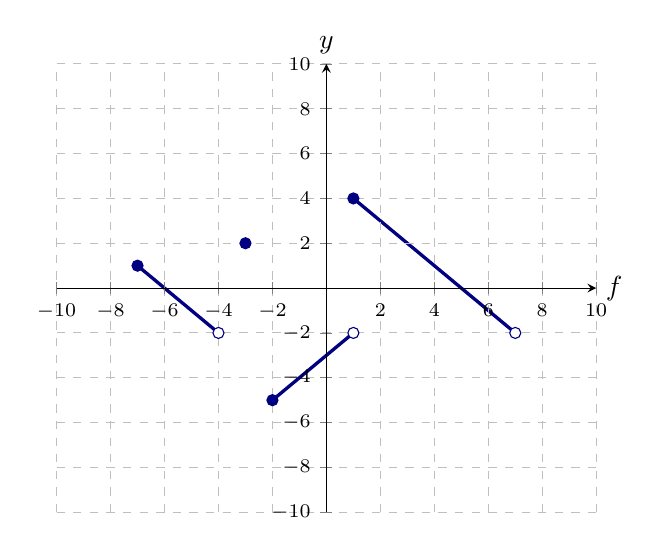
\begin{tikzpicture}
  \begin{axis}[
            domain=-10:10, ymax=10, xmax=10, ymin=-10, xmin=-10,
            axis lines =center, xlabel=$f$, ylabel=$y$, grid = major, grid style={dashed},
            ytick={-10,-8,-6,-4,-2,2,4,6,8,10},
            xtick={-10,-8,-6,-4,-2,2,4,6,8,10},
            ticklabel style={font=\scriptsize},
            every axis y label/.style={at=(current axis.above origin),anchor=south},
            every axis x label/.style={at=(current axis.right of origin),anchor=west},
            axis on top
          ]
          
  \addplot [draw=penColor,very thick,smooth,domain=(-7:-4)] {-x-6};
  \addplot [draw=penColor,very thick,smooth,domain=(-2:1)] {x-3};
  \addplot [draw=penColor,very thick,smooth,domain=(1:7)] {-x+5};

  \addplot[color=penColor,only marks,mark=*] coordinates{(-3,2)}; 
  
  \addplot[color=penColor,only marks,mark=*] coordinates{(-7,1)}; 
  \addplot[color=penColor,fill=white,only marks,mark=*] coordinates{(-4,-2)}; 
  \addplot[color=penColor,only marks,mark=*] coordinates{(-2,-5)}; 
  \addplot[color=penColor,fill=white, only marks,mark=*] coordinates{(1,-2)}; 
  \addplot[color=penColor,only marks,mark=*] coordinates{(1,4)}; 
  \addplot[color=penColor,fill=white,only marks,mark=*] coordinates{(7,-2)}; 


    \end{axis}
\end{tikzpicture}
\end{image}


$m$ has two zeros: $-6$ and $\answer{5}$. These are represented by intercepts in the left and right line segments. \\
$m$ has a global minimum represent by the left endpoint of the middle line segment. \\
$m$ has a global maximum represent by the left endpoint of the right line segment.





Graph of $z = P(t) = \frac{1}{2} \, m(t)$.

\begin{image}
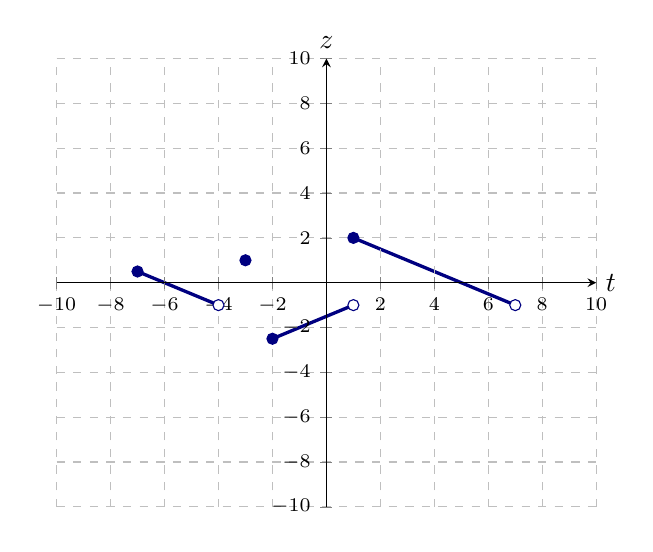
\begin{tikzpicture}
  \begin{axis}[
            domain=-10:10, ymax=10, xmax=10, ymin=-10, xmin=-10,
            axis lines =center, xlabel=$t$, ylabel=$z$, grid = major, grid style={dashed},
            ytick={-10,-8,-6,-4,-2,2,4,6,8,10},
            xtick={-10,-8,-6,-4,-2,2,4,6,8,10},
            ticklabel style={font=\scriptsize},
            every axis y label/.style={at=(current axis.above origin),anchor=south},
            every axis x label/.style={at=(current axis.right of origin),anchor=west},
            axis on top
          ]
          
  \addplot [draw=penColor,very thick,smooth,domain=(-7:-4)] {-0.5*(x+6)};
  \addplot [draw=penColor,very thick,smooth,domain=(-2:1)] {0.5*(x-3)};
  \addplot [draw=penColor,very thick,smooth,domain=(1:7)] {-0.5*(x-5)};

  
  
  \addplot[color=penColor,only marks,mark=*] coordinates{(-7,0.5)}; 
  \addplot[color=penColor,fill=white,only marks,mark=*] coordinates{(-4,-1)}; 
  \addplot[color=penColor,only marks,mark=*] coordinates{(-3,1)}; 
  \addplot[color=penColor,only marks,mark=*] coordinates{(-2,-2.5)}; 
  \addplot[color=penColor,fill=white,only marks,mark=*] coordinates{(1,-1)}; 
  \addplot[color=penColor,only marks,mark=*] coordinates{(1,2)}; 
  \addplot[color=penColor,fill=white,only marks,mark=*] coordinates{(7,-1)}; 


    \end{axis}
\end{tikzpicture}
\end{image}




\begin{itemize}

\item The domain of $P$ is $\left[\answer{-7},\answer{-4}\right) \cup \{3\} \cup [-2,7)$, equal to the domain of $m$. The domain remains the same, since the factor $\frac{1}{2}$ was outside the domain parentheses in the formula for $m$. The $\frac{1}{2}$ is multiplying the function values.
\item $P$ has two zeros: $-6$ and $5$. These are represented by intercepts in the left and right line segments. (Because, $\frac{1}{2} \cdot 0 = 0$.) \\
\item $P$ has a global minimum represented by the left endpoint of the middle line segment. \\
\item $P$ has a global maximum represented by the left endpoint of the right line segment.

\end{itemize}


\end{example}


Multiplying a function by a positive constant less than $1$ compresses the graph vertically.  Since compressing $0$ still gives $0$, the intercepts do not change.  Everything is compressed from the intercepts. The intercepts stay pinned where they are.
























\begin{example} Sine



Graph of $y = 3 \sin(\theta)$.

\begin{image}
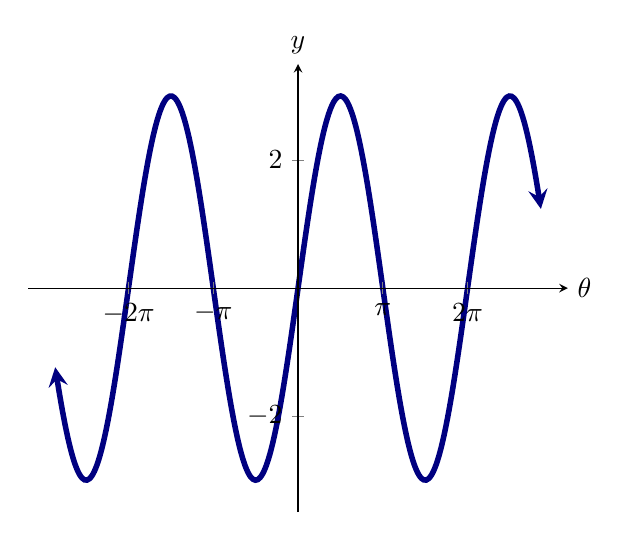
\begin{tikzpicture} 
  \begin{axis}[
            domain=-10:10, ymax=3.5, xmax=10, ymin=-3.5, xmin=-10,
            xtick={-6.28, -3.14, 3.14, 6.28}, 
            xticklabels={$-2\pi$, $-\pi$, $\pi$, $2\pi$},
            axis lines =center,  xlabel={$\theta$}, ylabel=$y$,
            every axis y label/.style={at=(current axis.above origin),anchor=south},
            every axis x label/.style={at=(current axis.right of origin),anchor=west},
            axis on top
          ]
          
          	\addplot [line width=2, penColor, smooth,samples=200,domain=(-9:9), <->] {3*sin(deg(x))};

           

  \end{axis}
\end{tikzpicture}
\end{image}


The location of zeros, maximums, and minimums inside the domain have not changed.  The function values have been multiplied by $3$. Therefore, the maximum and minimum values of the function have changed. But their positions have not.

\begin{itemize}
\item The zeros of $\sin(\theta)$ are all integer multiples of $\pi$.
\item The maximum value is $1$ and it occurs at:  $\left\{     \frac{(4k+1)\pi}{2} \, | \, k \in \textbf{Z}     \right\}$
\item The minimum value is $-1$ and it occurs at:  $\left\{    \frac{(4k+3)\pi}{2} \, | \, k \in \textbf{Z}     \right\}$
\end{itemize}













\end{example}






Neither shifting nor stretching (or compressing) changes the shape of the graph.  The extreme features may change their values, but they remain relatively in the same position.  The shape may be reflected about one (or both) of the axes, but the shape is the same, just drawn in reverse from the original.





\subsection*{Together}

We can apply horizontal and vertical stretches together as well.





\begin{example}  Shifting

Let $C(w) = \frac{1}{2}|3w|$.


\begin{image}
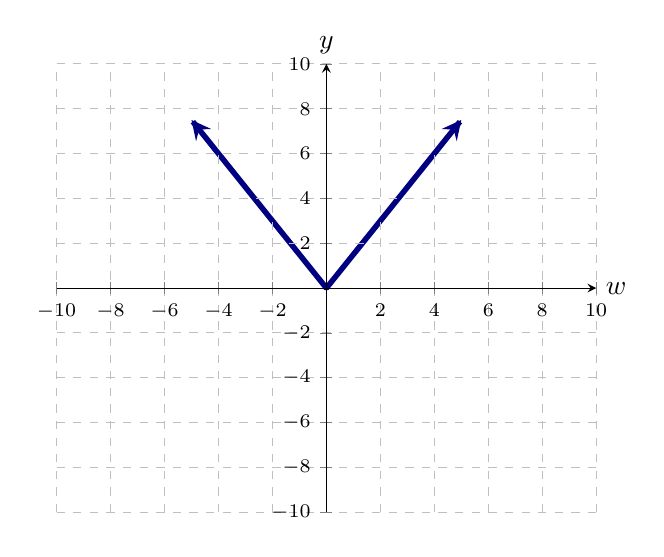
\begin{tikzpicture} 
  \begin{axis}[
            domain=-10:10, ymax=10, xmax=10, ymin=-10, xmin=-10,
            axis lines =center, xlabel=$w$, ylabel=$y$, grid = major, grid style={dashed},
            ytick={-10,-8,-6,-4,-2,2,4,6,8,10},
            xtick={-10,-8,-6,-4,-2,2,4,6,8,10},
            ticklabel style={font=\scriptsize},
            every axis y label/.style={at=(current axis.above origin),anchor=south},
            every axis x label/.style={at=(current axis.right of origin),anchor=west},
            axis on top
          ]
          
          \addplot [line width=2, penColor, smooth, samples=200, domain=(-5:5),<->] {0.5 * abs(3*x)};
        

  \end{axis}
\end{tikzpicture}
\end{image}

\end{example}

The graph of $|w|$ has been compressed horizontally by a factor of $\frac{1}{3}$ and compressed vertically by a factor of $\frac{1}{2}$.




We have already noticed that multiplication and addition on the inside of the formula's parentheses affect the domain.  They also have graphical effects which seem backwards from the arithmetic.  This is because the formula shows us what happens to the new domain variable, not the original variable.  We have to set the original variable equal to this new domain expression and solve for the new variable.  That tells us what happens to the original variable.  When we solve, all of the arithmetic is reversed and that is what we see graphically.

This is not the case for multiplication and addition on the outside of the parentheses.  The value of the formula is the value of the function, which gives the heights of the dots on the graph.  The multiplication and addition is applied directly to this value.  Therefore, the graphical effects follow the arithmetic.


\begin{center}

Graphs follow domain transformations backwards or in reverse as the arithmetic.


\end{center}


\begin{center}

Graphs follow range transformations exactly as the arithmetic.


\end{center}













\begin{center}
\textbf{\textcolor{green!50!black}{ooooo-=-=-=-ooOoo-=-=-=-ooooo}} \\

more examples can be found by following this link\\ \link[More Examples of Stretching]{https://ximera.osu.edu/csccmathematics/precalculus1/precalculus1/stretching/examples/exampleList}

\end{center}





\end{document}
